\chapter[Giant Number Fluctuations in 3-Dimensional Space]{Giant Number Fluctuations in 3-Dimensional Space}
\label{giant-number-fluctuations-in-3-dimensional-space}
%%%%%%%%%%%%%%%%%%%%%%%%%%%%%%%%%%%%%%%%%%%%%%%%%%%%%

\section{Introduction}
Active fluids exhibit many unusual behaviors beyond the expectation of equilibrium statistical mechanics \cite{Ramaswamy2010,Cates2012,Marchetti2013,Poon2013,Elgeti2015}.
In particular, an active fluid can exhibit anomalously large density variations, the so-called giant number fluctuations (GNF), where the standard deviation of the number of particles grows nonlinearly with the square root of the mean particle number, defying the central limit theorem of equilibrium systems \cite{Mishin2015}.
Such unusual density fluctuations have been observed in a wide range of active fluids in both living and non-living systems including vibrated granular rods \cite{Narayan2007,Aranson2008,Kudrolli2008,Deseigne2010},
swarming bacteria \cite{Zhang2010,Nishiguchi2017} and mammalian cells \cite{Kawaguchi2017},
self-propelled cytoskeleton \cite{Schaller2013}, and synthetic colloidal swimmers \cite{Palacci2013,Karani2019}. As a result, GNF has generally been viewed as a hallmark of the emergent behaviors of active fluids.


Significant theoretical and computational advancement on GNF has been made over the past two decades since the seminal works of Toner and Tu \cite{Toner1995,Tu1998,Toner1998,Simha2002,Ramaswamy2003,Toner2005,Chate2008,Mishra2010,
Dey2012,Saintillan2012,Saintillan2013,Ngo2014,Mahault2019}. Meanwhile, many important theoretical and numerical predictions have been tested in experimental realizations
\cite{Narayan2007, Aranson2008, Deseigne2010, Zhang2010, Schaller2013,
Nishiguchi2017, Kawaguchi2017, Palacci2013}.

Of particular interest is the scaling exponent $\alpha$, which is defined following $\Delta N /\sqrt N \propto N^\alpha$, where $\Delta N$ is the standard deviation of particle number and $N$ is the mean number of particles in a subsystem of given size. Heretofore, all the existing experiments on GNF were limited to two-dimensional (2D) or quasi-2D systems. In contrast to theoretical predictions (where $\alpha \approx 0.3$), $\alpha$'s obtained in these experiments show large variations ranging from 0.13 to 0.5. Such a large variation arises partially because of complicated particle-boundary interactions, which are hard to incorporate in theoretical studies. Moreover, the predictions of $\alpha$ in three-dimensional (3D) wet active fluids---one of the most important classes of active fluids where hydrodynamics dominate the interparticle interactions and conserve the total momentum of systems \cite{Marchetti2013}---has not been experimentally testified. Therefore, there is an imperative need for an experimental measurement of $\alpha$ in 3D active fluids, which are not affected by system boundaries. Such a measurement will provide not only an unambiguous experimental benchmark to testify theories of active fluids, but also experimental support on the effect of dimensionality on GNF of active fluids \cite{Marchetti2013}.

The rise of GNF in active fluids is usually accompanied by the transition to ordered phases with collective motions \cite{Ramaswamy2010,Marchetti2013}. For wet 3D active fluids such as bacterial suspensions, these collective motions lead to large-scale coherent flows with intermittent vortices and jets, which are often referred to as active turbulence \cite{Wolgemuth2008,Wensink2012,Dunkel2013a,Bratanov2015,Guo2018,Linkmann2019,Bardfalvy2019,Alert2020,Skultety2020,Peng2020}. Similar to GNF that manifests density fluctuations across different scales, the flow of active turbulence also exhibits scale-dependent structures.
Imported from the study of classical turbulence, energy spectra are frequently measured to quantify such structures in active turbulence \cite{Ishikawa2011,Wensink2012,Dunkel2013a,Giomi2015,Creppy2015,Patteson2018,Alert2020}. Although both GNF and energy spectra quantify the scale-dependent dynamics of active fluids, the deep connection between these two quantities at different scales has not been experimentally investigated. Our experiment reveals the density- and scale- independent coupling between GNF and energy spectra, suggesting that GNF is governed by the strength of the motion-induced flow.

\begin{figure}[!h]
\begin{center}
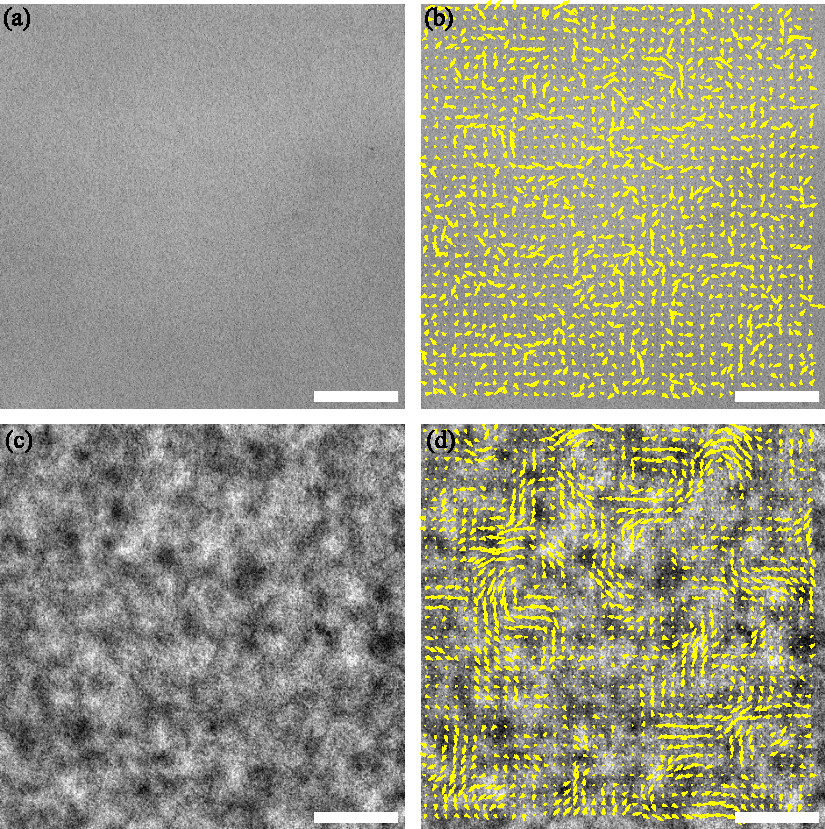
\includegraphics[width=5.5in]{figs/5-GNF/1.pdf}
\caption[Images of bacterial active turbulence and its flow fields]
{
\textbf{Images of bacterial active turbulence and its flow fields.}
(a) and (b) are active turbulence in a dense bacterial suspension (6.4\%) displaying constantly varying concentration inhomogeneity and the corresponding flow field.
(c) and (d) are a dilute bacterial suspension (1.6\%) and the corresponding flow field.
Scale bars are 85 $\mu$ m.
}
\label{fig:experiment}
\end{center}
\end{figure}


\section{Methods}

\subsection{Sample preparation, imaging and routine analysis}
Here, we present our systematic experimental study of GNF and energy spectra in bulk bacterial suspensions, a premier example of 3D wet active fluids. We use genetically engineered light-powered \textit{Escherichia coli} (\textit{E. coli}) as our model bacteria.
For a typical experiment, a bacterial suspension of control volume fraction $\phi$ is injected into a sealed chamber of 20 mm $\times$ 3 mm $\times$ 140 $\mu$m.
Without supply of oxygen, bacteria quickly consume all the remaining oxygen in the chamber and stop moving after $5$ minutes.
We then illuminate the suspension with a high-intensity microscope light, which powers bacteria at their maximal swimming speed of $15 \pm 3$ $\mu$m/s in the dilute limit.
A video of the suspension is taken 50 $\mu$m above the bottom wall of the chamber by a bright-field inverted microscope at a frame rate of $30$ fps and the field of view of $420 \times 360$ $\mu$m$^2$ (Fig.~\ref{fig:experiment}a, c).
We use a standard Particle Image Velocimetry (PIV) algorithm \cite{OpenPIV-website}
to extract the 2D in-plane velocity field $(v_x,v_y)$ in the 3D suspension, which exhibits the characteristic chaotically-moving vortices and jets of active turbulence at high $\phi$ (Fig.~\ref{fig:experiment}b, d).

\subsection{Relation between pixel intensity and concentration}

It is challenging to directly count the number of bacteria in a 3D suspension of fasting moving bacteria. Luckily, by virtue of Beer-Lambert law, the local bacterial density is monotonically correlated with the local intensity of microscope images, where darker regions correspond to higher bacterial densities (Fig.~\ref{fig:experiment}c). Similarly principles also appeared in other experimental works, where optical information was exploited in probing the dynamics in suspensions of bacteria and actin filaments \cite{Sokolov2009, Wilson2011, Schaller2013}.

\begin{figure}[!]
\begin{center}
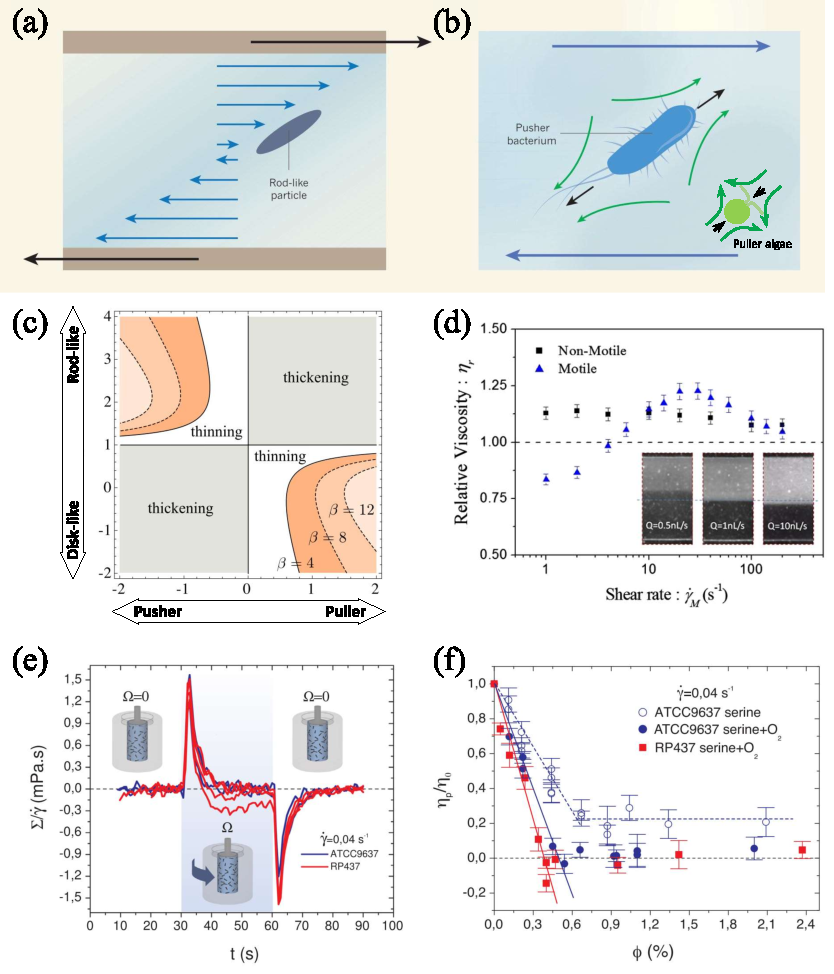
\includegraphics[width=3.5in]{figs/5-GNF/2.pdf}
\caption[Relation between image intensity and concentration]
{
\textbf{Relation between image intensity and concentration.}
(a) Images of bacterial suspensions of different volume fractions under the same illumination conditions.
(b) Volume fractions as a function of average pixel intensities.
}
\label{fig:calibration}
\end{center}
\end{figure}

To calibrate the density-intensity correlation, we prepare bacterial suspensions of different $\phi$ and image the suspensions under the same illumination (Fig.~\ref{fig:calibration}a). The mean image intensity decreases with increasing $\phi$ following an approximately linear relation (Fig.~\ref{fig:calibration}b), agreeing with the the Beer-Lambert law for samples of small thickness and weak absorptivity appropriate for our experiments. The linear density-intensity relation has also been used in previous experiments on \textit{E. coli} suspensions \cite{Wilson2011}.

In the low attenuation limit (small thickness and weak absorptivity), $I=I_0-\epsilon$ where $\epsilon\ll I_0$:
\begin{equation}
  \log \frac{I_0}{I} = \log \frac{I_0}{I_0 - \epsilon} \approx \frac{\epsilon}{I_0} \sim c
\end{equation}
\begin{equation}
I = I_0 - \epsilon \sim c
\end{equation}
where $I_0$ is the original light intensity, $I$ is the transmission light intensity, $\epsilon$ is the attenuated light intensity, which is much smaller than the original light intensity.

\begin{figure}[!]
\begin{center}
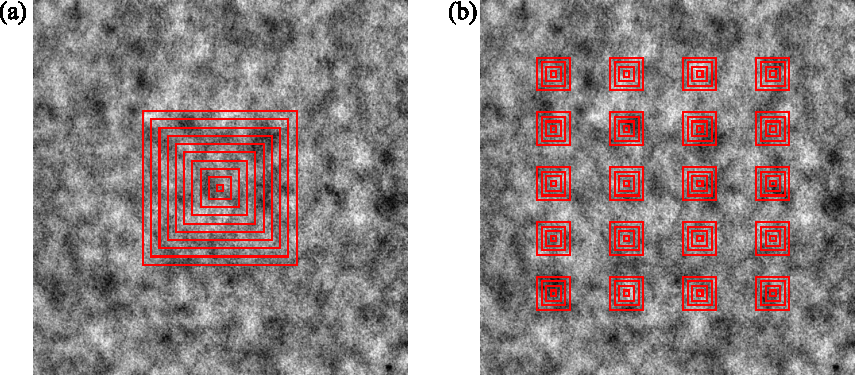
\includegraphics[width=0.9\textwidth]{figs/5-GNF/GNF-calculations.pdf}
\caption[GNF calculations]
{
\textbf{GNF calculations.}
(a) Varying subsystem sizes.
(b) Multiple seeds of subsystems for spatial average.
}
\label{GNF-calculation}
\end{center}
\end{figure}

\subsection{GNF calculations}

The basic principle of measuring GNF is to get the scaling exponent of the standard deviation of the number of particles $\Delta N$ against the mean number $N$. We adopt the temporal variance \& spatial average (TVSA) method to do the calculation.

Two methods have been used to quantify giant number fluctuations. Both divide the whole system into many small subsystems. Then, one of them calculates the mean number $N$ and standard deviation $\Delta N$ over time, and then average spatially (temporal variance -\> spatial average, TVSA) \cite{Narayan2007}. The other calculates $N$ and $\Delta N$ over all the small subsystems in one frame, then takes an average over time (spatial variance -\> temporal average, SVTA) \cite{Aranson2008}.

Urbach 2008 futher stated that when a system is homogeneous, where spatial and temporal correlations are small compared with the system size and experiment duration, two methods give the same result. Our experimental system, \textit{E. coli} suspensions, has a correlation length ($\sim 30$ \textmu m) much smaller than the system size ($\sim 140$ \textmu m), and is thus a spatially homogeneous system. If observed over a sufficiently long time (longer than the autocorrelation time), the system can be regarded as being temporally homogeneous as well.

In real experiment, we rely on image pixel intensity to measure local concentrations. The illumination light in our microscope system, and probably all microscope systems, presents a slight inhomogeneity which is quite stable and long-standing. This has caused trouble when we tried to use the second method (SVTA) to measure GNF (show a figure of GNF in stationary samples). In principle, such inhomogeneity can be removed by a removing the background preprocessing. However, without enough images for a sample, such a preprocessing may lead to larger errors. As a result, we adopt the TVSA method, which is not sensitive to the long-standing spatial inhomogeneity and works more robustly in our measurement. A way to understand the fact that TVSA is not sensitive to illumination inhomogeneity is to think of it as adding a constant image to each frame, which does not affect the temporal variation calculation.

The TVSA method starts by cropping square-shape subsystems of various sizes from the original image time series, as shown in Fig.~\ref{GNF-calculation}a. For each size $l$, a standard deviation $\Delta N$ and a mean $N$ are calculated over the time series. In order to add more statistics to the data extracted from a time series, we choose 20 evenly distributed spots (Fig.~\ref{GNF-calculation}b) as the seeds of the subsystems and average the results calculated from all these subsystems to give the result for a video. We vary the subsystem size $l$ from 10 \textmu m to 30 \textmu m, and examine the temporal variations (standard deviations) of bacterial concentrations $\Delta N_{ij}$ in the $i^{th}$ frame for each box size $l_j$. The temporal variations are then averaged in space (over $i$) to give a single value variation $\Delta N_{j}$.
Then number fluctuations in the system is captured by the dependence of $\Delta N_{j}$ on $l_j$. In an equilibrium system, $\Delta N_{j}\propto l_j$ (this follows from $\Delta N_{j}\propto \sqrt{N_j}$ and $N_j\propto l_j^2$).
Thus, the deviation from $\Delta N_{j}\propto l_j$ quantifies the giant number fluctuation in the system.
In the main paper, we plot $\Delta N_{j}/l_j$ as a function of $l_j^2/l_b^2$, where $l_b$ is the length scale of single bacterial body length, chosen to be 3 \textmu m.
To be consistent with the notations in literatures, we get rid of the subscript $j$, and write $l_j$ as $\sqrt{N}$.
Note that the subscript $j$ denotes different choices of box sizes.

Without a more careful calibration, we are not able to obtain the exact number of particles using this Beer's law based method. Fortunately, the calculations of GNF does not require the exact number, but only the relative number. In the main paper, we show that the volume fractions $\phi$ and average pixel intensities $I$ follow a pretty linear relation. Such a relation entails that $\Delta I \propto \Delta N$, which is followed by $\Delta I/\sqrt N \propto \Delta N/\sqrt N$. The proportionality allows us to get the scaling exponents of $\Delta N/\sqrt N$ against $N$, without having to measure the exact particle numbers.

\begin{figure}[!h]
\begin{center}
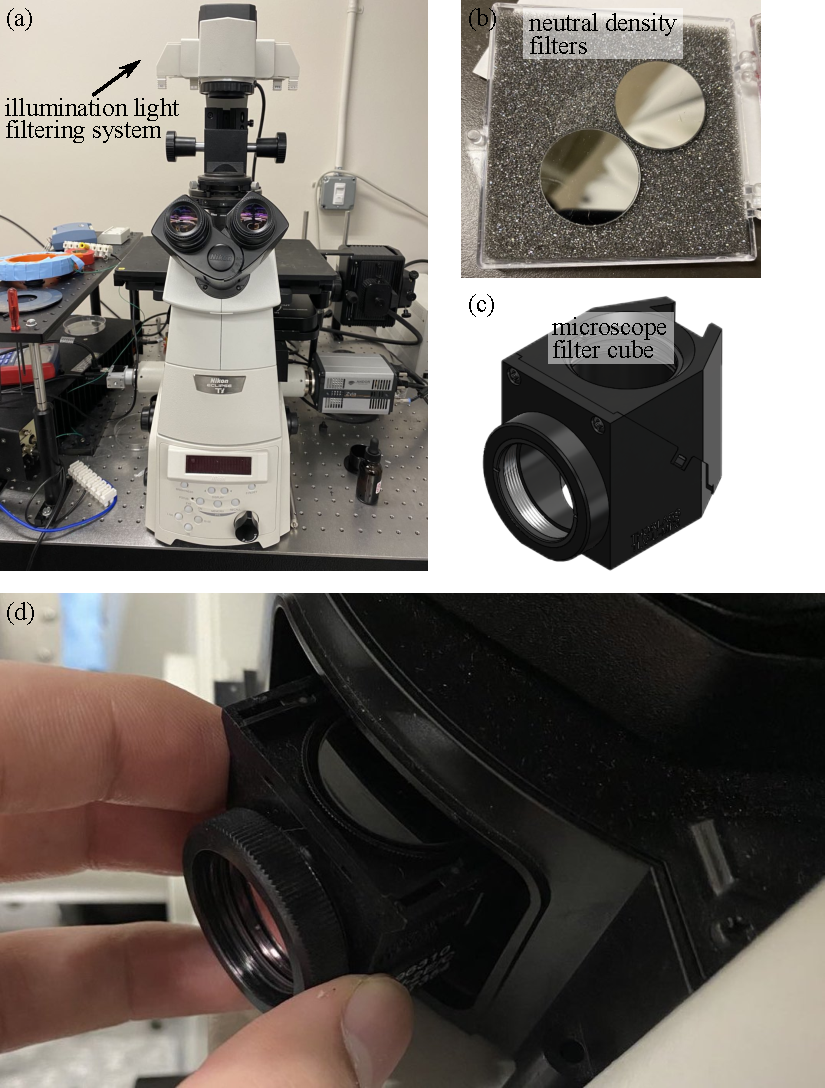
\includegraphics[width=4.5in]{figs/5-GNF/3.pdf}
\caption[Spatial and temporal correlation functions in active turbulence]
{
\textbf{Spatial and temporal correlations functions of density and velocity in active turbulence.}
(a) and (b) are density spatial correlation functions and autocorrelation functions.
(c) and (d) are velocity spatial correlation functions and autocorrelation functions.
(e) Correlation lengths of both density and velocity correlation functions, defined as the distance $\lambda$ where $C_{n(v)}(\lambda)=1/e$.
(f) Autocorrelation times of both density and velocity autocorrelation functions, defined as the time $\tau$ where $C_{n(v)}(\tau)=1/e$.
}
\label{fig:spatiotemporal-correlations}
\end{center}
\end{figure}

\subsection{Cross correlation}

The cross correlation calculation used when analyzing the local correlation between kinetic energy and density fluctuations is defined as the following:
\begin{equation}
\label{eq:cross-correlation}
A\star B = \frac{\langle(A-\bar A)(B-\bar B)\rangle}{\sigma_A\sigma_B}
\end{equation}
where $A$ and $B$ are two arrays of scalars, $\star$ is the operator standing for cross correlation, $\bar\cdot$ means taking the mean, $\sigma$ means the standard deviation, and $\langle\cdot\rangle$ denotes taking the average of all scalars in an array. The cross correlation quantifies the similarity between arrays $A$ and $B$. The resulting number takes value from -1 to 1.

\subsection{Energy spectra}

We calculate the energy spectra using the following formula
\begin{equation}
E(k_x, k_y) = \frac{\langle u_k(k_x, k_y)u^*_k(k_x, k_y)+v_k(k_x, k_y)v_k^*(k_x, k_y)\rangle}{2A}
\end{equation}
where $E$ is the energy density in $k$ space, $u_k$ and $v_k$ are $k$ space velocity fields, $A$ is the real space area of the system and $^*$ denotes the complex conjugate. The $\langle\cdot\rangle$ denotes an average over multiple images from different times.

\section{Results}
\subsection{Density fluctuations}

The simple linear relation allows us to measure the spatiotemporal evolution of relative local bacterial densities and investigate density fluctuations in 3D bacterial suspensions. We first calculate the two-point density spatial correlation and the density auto-correlation for suspensions of different $\phi$ and compare them with well-studied velocity correlations extracted from PIV (Fig.~\ref{fig:spatiotemporal-correlations}).

The correlation length $\lambda$ and correlation time $\tau$ are determined when the corresponding normalized correlation functions decay to $1/e$ (Fig.~\ref{fig:spatiotemporal-correlations}c, f). Fig.~\ref{fig:spatiotemporal-correlations}c shows the density correlation lengths at different $\phi$, which characterize the scale of density inhomogeneities in suspensions.
$\lambda$ is small at low $\phi$, gradually increases with $\phi$ and reaches a plateau of $\sim 5l_b$ in high-concentration bacterial suspensions of $\phi > \phi_c = 3.5\%$, where $l_b=3$ $\mu$m is the average length of bacterial body. The velocity correlation length follows the exact same trend and also saturates when $\phi > \phi_c$. Such a quantitative similarity indicates the direct coupling between density fluctuations and collective turbulent flows, a feature we shall examine in much more details later. In the fully-developed turbulent regime above $\phi_c$, the velocity correlation length is about twice of the density correlation length.
Fig.~\ref{fig:spatiotemporal-correlations}f shows the density and velocity correlation times at different $\phi$. The velocity and density correlation time at low $\phi$ show a large discrepancy. When $\phi > \phi_c=3.5\%$, they plateau at $\sim 6\tau_b$ and $\sim 4\tau_b$, respectively, where $\tau_b=0.2$ s is the characteristic time scale of \textit{E. coli} swimming.
% I don't know how to interpret the large difference in \tau at low concentration. It may be due to the dominanace of illumination light at low concentration.


\begin{figure}[!h]
\begin{center}
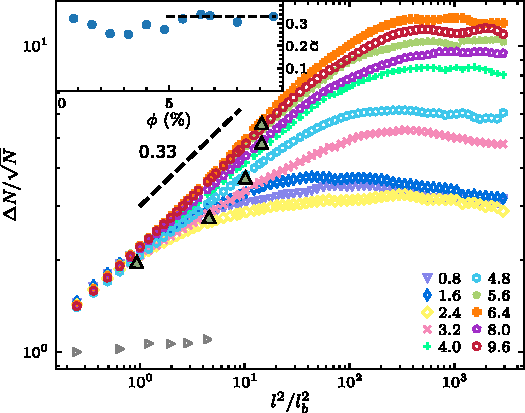
\includegraphics[width=4.5in]{figs/5-GNF/4.pdf}
\caption[Giant number fluctuations in active turbulence]
{
Standard deviation of particle number $\Delta N$ scaled by particle mean number $N$ plotted against subsystem size rescaled by single bacterium size $l^2/l_b^2$ in bacterial suspensions at volume fractions ranging from 0\% to 9.6\%. Dark green triangles indicates the density correlation lengths at each volume fraction. Black dashed line is a guide of the eye with power 0.33. Inset: scaling exponents $\alpha$ at different volume fractions. All $\alpha$'s are fitted from 0.3 $l_b$ to the correlation lengths. Dashed line in the inset indicates $\alpha=0.33$.
}
\label{fig:GNF}
\end{center}
\end{figure}

We further examine GNF by calculating the standard deviation of bacterial number $\Delta N$ and the mean bacterial number $N$ in subsystems of increasing sizes. $\Delta N / \sqrt N$ as a function of $l^2/l_b^2$ for bacterial suspensions of different $\phi$ is plotted in Fig.~\ref{fig:GNF}, where $l$ is the side length of square subsystems.
Note that the area of the subsystem $l^2$ is linearly proportional to mean particle number $N$ at given $\phi$. At small length scale, when $l\le\lambda_n$, bacterial suspensions of all volume fractions examined in this study (1.2\% to 14.4\%) exhibit GNF, with $\Delta N/\sqrt N$ increasing with subsystem size $l^2$. When the size of subsystems is much larger than the density correlation length $\lambda$, the giant fluctuation diminishes due to the spatial average over multiple dense and dilute regions.

The degree of GNF can be quantified by the scaling exponent $\alpha$ following $\Delta N/\sqrt{N} \sim N^\alpha$. $\alpha=0$ for equilibrium systems obeying the central limit theorem, whereas the upper bound $\alpha = 0.5$ corresponds to a system with maximal density fluctuations.
We extract $\alpha$ by fitting the experimental curves with power-law relations only below the density correlation length $\lambda$. The inset of Fig.~\ref{fig:GNF} shows $\alpha$ as a function of $\phi$.

At all volume fractions, $\alpha$ takes a value of $0.30 \pm 0.03$. Notably, at high volume fractions, when $\phi \geq \phi_h = 6.4\%$, $\alpha$ approaches a narrower plateau of $0.33 \pm 0.01$.

The plateau value quantitatively agrees with the theoretical prediction of $\alpha = 1/3$ for 3D suspensions of polar-ordered self-propelled particles with hydrodynamic interactions \cite{AditiSimha2002}. As such, our experiments provide the first quantitative verification of the theory of GNF in 3D wet active fluids.

The observation of GNF at volume fractions lower than $\phi_c$ suggests that even in a dilute suspension below the turbulent transition, bacteria swim in a correlated fashion, in qualitative agreement with the prediction of the kinetic theory \cite{Stenhammar2017}.


\begin{figure}[!h]
\begin{center}
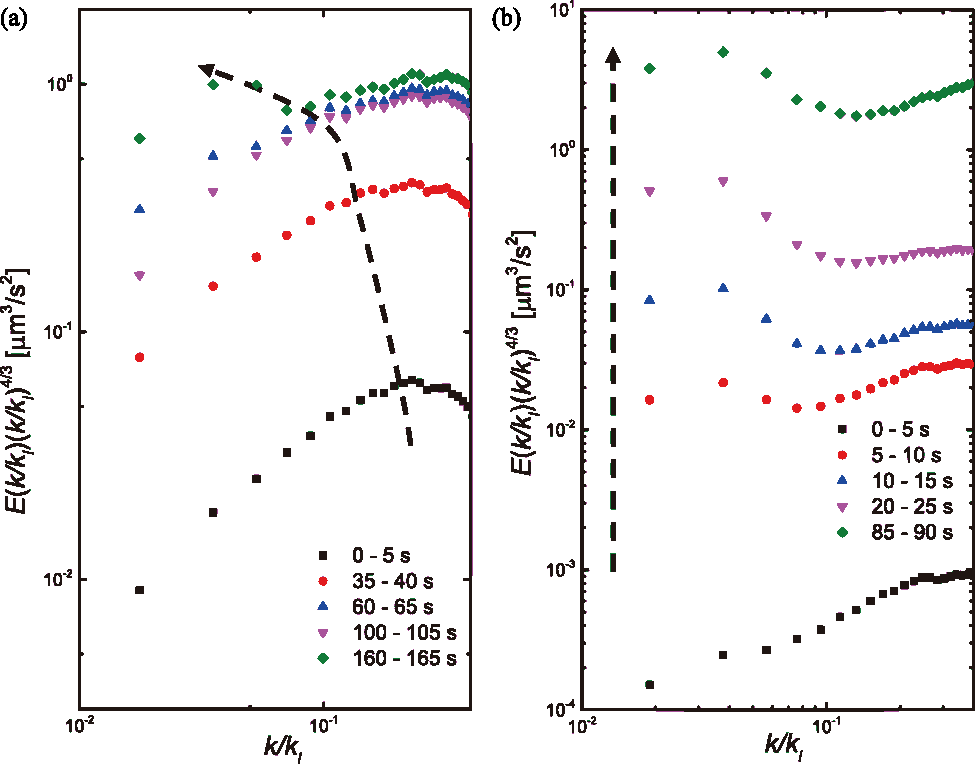
\includegraphics[width=4.5in]{figs/5-GNF/5.pdf}
\caption[Energy spectra in active turbulence]
{
Energy spectra of bacterial active turbulence at volume fractions ranging from 0.8\% to 9.6\%. Shaded region indicates the range over which the scaling exponents $\beta$ are fitted. Red dashed line is a fitting of the $\phi=0.8\%$ curve (purple), based on the hydrodynamic model of Ref.~\cite{Bardfalvy2019}. Fitting parameters: $n=0.02\%$.
Inset: Scaling exponents of energy spectra ($\beta$) as a function of volume fractions $\phi$. Dashed line is $\beta=3.3$.
}
\label{fig:energy-spectra}
\end{center}
\end{figure}


\subsection{Energy spectra}

Similar to GNF, the velocity field of active turbulence also shows scale-dependent structures, which are often characterized by the energy spectrum of turbulent flows, $E(k)$ \cite{Liu2020}. $E(k)$ measures the kinetic energy density at different scales in terms of wavenumber $k = 2\pi/l$. It is related to the mean kinetic energy density $E = \langle v_x^2 + v_y^2 \rangle/2$ via $E = \int_0^\infty E(k)dk$. Fig.~\ref{fig:energy-spectra} shows $E(k)$ of bacterial suspensions at different $\phi$. The low $\phi$ energy spectrum has been theoretically predicted for uncorrelated pusher swimmers \cite{Bardfalvy2019} as Eq.~\ref{eq:energy-spectra}
\begin{equation}
\label{eq:energy-spectra}
E_k = 4\pi n \kappa^2 \left[ \frac{1}{3} + \frac{\cos(kl)}{(kl)^2} - \frac{\sin(kl)}{(kl)^3} \right] \frac{\epsilon^4k^2}{l^2} K_2^2(k\epsilon)
\end{equation}
where  $\kappa \approx 400$ $\mu$m$^3$/s is the dipole strength of \textit{E. coli}, $l\approx 1.9$ $\mu$m is the dipolar length, $\epsilon$ is a factor describing the distance over which the regularisation acts and $K_2$ is the modified Bessel function of the second kind. The red dashed curve in Fig.~\ref{fig:energy-spectra} shows the best fitting of our experimental data with the theoretical prediction. As can be seen, the low $\phi$ prediction of $E(k)$ quanlitatively agrees with our measurements.
Particularly, $E(k)$ is flat in the small $k$ limit, a feature arising from the superposition of the dipolar flow fields of uncorrelated bacteria \cite{Bardfalvy2019}. However, the fitting parameter $n$ for the best fitting is found to be 0.02\%, 40 times smaller compared to the parameter in real experiment. % suggesting that?

With increasing $\phi$, $E(k)$ at small $k$ increases sharply. In the turbulent regime at high $\phi$, the kinetic energy is all concentrated at scales much larger than the size of single bacteria $l_b$, even though the turbulent flows are completely powered by single bacterial swimming at $l_b$. % manifesting long-wave instability?
Weak peaks are observed for high $\phi$ suspensions at low $k$. This overall trend of $E(k)$ with increasing $\phi$ qualitatively agrees with large-scale simulations \cite{Saintillan2012,Bardfalvy2019}.

We also extract the scaling exponent $\beta$ from $E(k) \sim k^{-\beta}$ by fitting the energy spectra at intermediate and large $k$ (between 0.03$k_b$ and 0.09$k_b$), where a significant change of $E(k)$ with $\phi$ occurs and $E(k)$ exhibits good power-law relations.
Similar to the trend of $\alpha$, $\beta$ also increases with $\phi$ and saturates at $3.2 \pm 0.1$ at high $\phi \geq \phi_h$. The saturated scaling exponent is quantitatively the same as that of the active turbulence of high-concentration suspensions of sperm at large $k$ \cite{Creppy2015}.
The exponent is also consistent with experiments on confined dense suspensions of \textit{B. subtilis} and swarming \textit{S. marcescens} on agar substrates, where the scaling of $E(k) \sim k^{-8/3}$ has been reported at large $k$ \cite{Wensink2012,Patteson2018}.
Since the characteristic vortex size quantified by the velocity correlation length is linearly proportional to the system size $L$ \cite{Guo2018}, when $k$ is significantly smaller than $2\pi/L$, $E(k)$ would decreases, exhibiting the non-monotonic trend shown in \cite{Wensink2012,Patteson2018}. The large system size of $L = 140$ $\mu$m of our experiments allows us to probe the small $k$ limit predicted by theories and simulations without the influence of system boundaries.

% haven't made any change on this part
Although the scaling in the small $k$ limit is strongly affected by the system size, the scaling in the large $k$ limit seems to be universal with $\beta \approx 3$ from different experiments. To the best of our knowledge, no theoretical prediction has been made on this interesting scaling behavior for 3D wet active fluids. Giomi investigated the energy spectra of 2D active nematics by combining numerical simulations with mean-field theories and showed $E(k) \sim k^{-4}$ in the large $k$ limit \cite{Giomi2015}.
The result has also been confirmed recently by a hydrodynamic theory \cite{Alert2020}. For isotropic turbulence in $d$ dimension, the energy spectra can be written as $E(k) = C_d k^{d-1} \langle \mathbf{v}(\mathbf{k})\cdot \mathbf{v}(-\mathbf{k})\rangle_{k = |\mathbf{k}|}$ \cite{Wensink2012,Bardfalvy2019},
where $C_d k^{d-1}$ is the surface area of $d$-sphere and $\langle \mathbf{v}(\mathbf{k})\cdot \mathbf{v}(-\mathbf{k})\rangle_{k = |\mathbf{k}|}$ is the Fourier transform of the velocity-velocity spatial correlation function. If we assume that the velocity correlation function for 2D active nematics is quantitatively similar to that of 3D bacterial suspensions independent of the dimensionality of systems, the mean-field theory would then predict the correct scaling of $E(k) \sim k^{-3}$ for 3D active turbulence. This hypothesis is certainly highly non-trivial and needs further theoretical investigation. Note that although we measure the energy spectra of 2D in-plane flows of 3D suspensions, the scaling of the spectra is the same as the spectra of 3D turbulent flows \cite{Pope2000}. Taken together, our study provides the first systematic experiments on the evolution of $E(k)$ over a large range of $\phi$ in bulk bacterial suspensions. The results quantitatively verify the existing theory on low-concentration active fluids and serve as a crucial benchmark for future theoretical development on the spectral properties of 3D active turbulence.


\begin{figure}[!]
\begin{center}
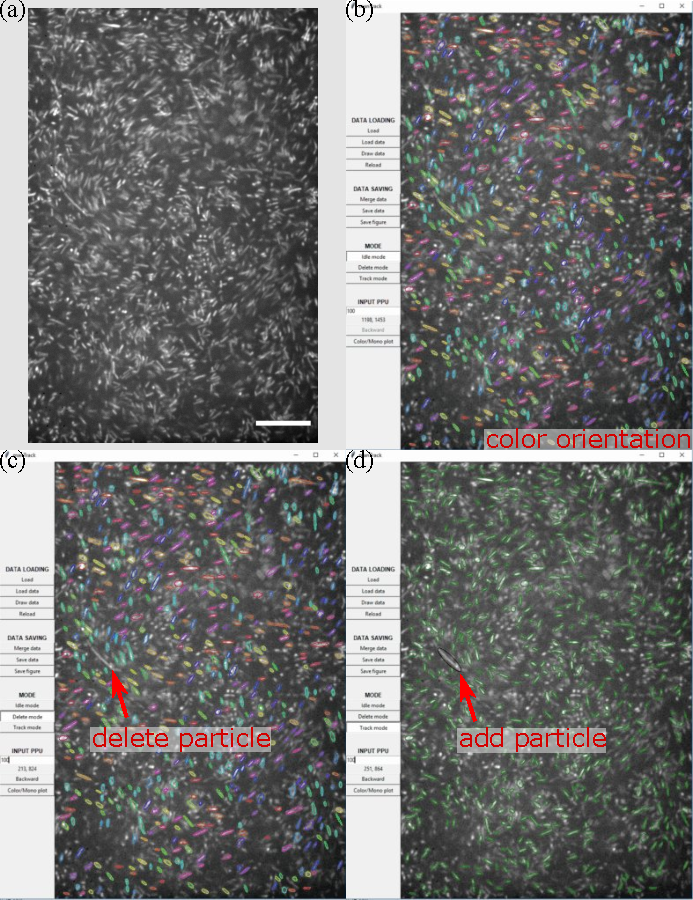
\includegraphics[width=4.5in]{figs/5-GNF/6.pdf}
\caption[The coupling between GNF and kinetic energy spectra]
{
\textbf{The coupling between GNF and kinetic energy spectra.}
(a) Energy spectra $E$ plotted against number fluctuations ($\Delta N/\sqrt N$) at corresponding length scales at volume fractions ranging from 0.8\% to 9.6\%. Black dashed line is a phenomenological fitting of the universal coupling between GNF and energy spectra across different volume fractions ($\log E = 2.2 (\log G)^2 - 4.8 \log G + 6.3$, where $G=\Delta N/\sqrt N$). Black arrow indicates the direction of increasing length scale, the hidden variable in this plot.
(b) Local correlations $C$ between density fluctuations and kinetic energy at volume fractions ranging from 0\% to 9.6\%. The correlations are calculated by averaging over 1000 frames. Inset: a snapshot of a density fluctuation field and a kinetic energy field.
}
\label{fig:GNF-energy-spectra-correlation}
\end{center}
\end{figure}


\subsection{Density-flow coupling}

Both GNF and energy spectra probe the scale dependence of active turbulence. The former measures density fluctuations at different scales, whereas the latter considers flow energies across scales. Although both properties have been extensively studied, the coupling between the two has not been explicitly examined so far.
The GNF curves and energy spectra shown in Fig.~\ref{fig:GNF} and \ref{fig:energy-spectra} show similar characteristics, including the rapid increase at small length scale and plateaus at large length scale. Such similarity suggests that a density-independent correlation between density fluctuations and kinetic energies may exist across all different length scales.
Indeed, when we plot density fluctuations $\Delta N/\sqrt N$ against the corresponding kinetic energies $E$ at the same scale in Fig.~\ref{fig:GNF-energy-spectra-correlation}a, all the $\Delta N/\sqrt N$-$E$ pairs fall onto a universal curve over two orders of magnitude in scales extending from the size of single PIV boxes to the vortex size in the turbulent regime, regardless of the specific volume fractions of the samples.
In contrast, $\Delta N/\sqrt N$-$E$ shows much larger scattering for low $\phi$ suspensions with random swimming bacteria.
Although it is not surprising that density fluctuations correlate with kinetic energies in general as both measure different aspects of the same active turbulence, the collapse of data from samples of different volume fractions is still quite unexpected.
The results show that the coupling between density fluctuations and turbulent flows occur at every scale of active turbulence in a quantitative same fashion. Such a scale-invariant coupling is independent of the volume fraction of bacterial suspensions. A phenomenological fitting of the universal coupling between density fluctuations and kinetic energy is shown in Fig.~\ref{fig:GNF-energy-spectra-correlation}a by a black dashed line.

To further illustrate such an unusual coupling in real space, we measure the \emph{local} correlation of density fluctuations and kinetic energy at a randomly chosen small scale of $l = 2.5l_b$. The local density fluctuation $\delta N(\mathbf{r},t)$ and local kinetic energy $E(\mathbf{r},t)$ at position $\mathbf{r} = (x,y)$ and time $t$ are extracted from the image intensity field and the PIV velocity field, respectively (Fig.~\ref{fig:GNF-energy-spectra-correlation}b inset).
The normalized correlation between $\delta N(\mathbf{r},t)$ and $E(\mathbf{r},t)$ is then computed at different $\phi$ (Fig.~\ref{fig:GNF-energy-spectra-correlation}b). At low $\phi$ with random swimming bacteria, the correlation is weak fluctuating around zero, which then increases with $\phi$ as bacterial suspensions transition to active turbulence. A constant positive correlation is found in the turbulent regime when $\phi \geq \phi_c$. The real-space measurement provides a concrete example of the coupling between density fluctuations and turbulent flows at small scales.

\begin{figure}[!]
\begin{center}
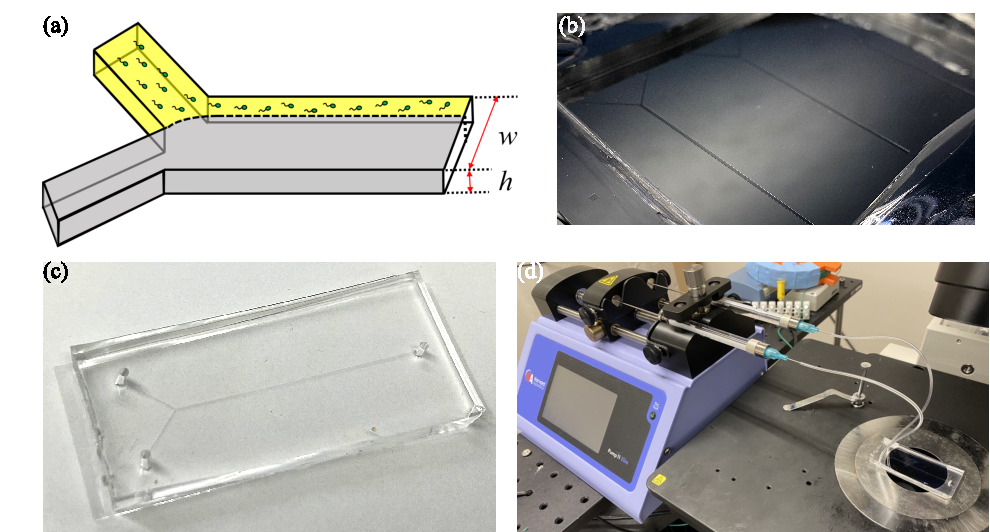
\includegraphics[width=5.5in]{figs/5-GNF/7.pdf}
\caption[Temporal evolution of $\alpha$, overall flow energy $E$ and fraction of aligned flow region $M$]
{
\textbf{Temporal evolution of $\alpha$, overall flow energy $E$ and fraction of aligned flow region $M$.}
(a) Snapshots of a bacterial suspension ($\phi=6.4\%$) during the transition towards active turbulence, overlaid with velocity fields obtained from PIV analysis. At $t=0$ s, we turn on the illumination light and the bacteria start to gain speed. Time are labeled in corresponding images.
(b) Temporal evolution of scaling exponent $\alpha$, total kinetic energy $E$ and the region fraction of aligned velocity $M$ in the same sample.
}
\label{fig:alpha-kinetics}
\end{center}
\end{figure}


Moreover, we find the same density-independent coupling in the kinetic process during the transition towards bacterial turbulence. Taking the advantage of the light-powered bacteria, we trigger the onset of bacterial turbulence by suddenly turning on the light illumination on high-concentration bacterial suspensions at $t=0$ \cite{Peng2020}. The density fluctuations and the energy spectra are then monitored as a function of $t$ before the suspensions reach the steady turbulent state.

\begin{figure}[h]
\begin{center}
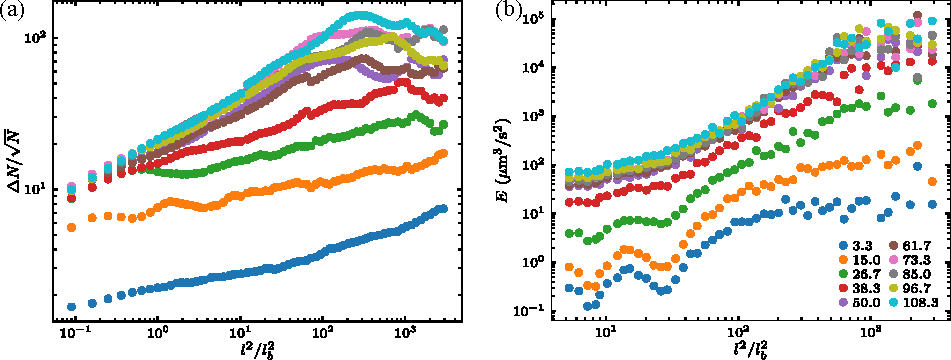
\includegraphics[width=5.5in]{figs/5-GNF/8.pdf}
\caption[GNF kinetics and energy spectra evolution over time during the transition towards active turbulence]
{
\textbf{GNF kinetics and energy spectra evolution over time during the transition towards active turbulence.} (a) Evolution of GNF. (b) Evolution of energy spectra. This particular sample has a volume fraction $\phi=6.4$. Different colors indicate different times. Values are shown as legends in (b), in unit of seconds.
}
\label{fig:GNF-energy-spectra-kinetics}
\end{center}
\end{figure}

Fig.~\ref{fig:alpha-kinetics}a shows 3 snapshots of a dense bacterial suspension during the transition towards active turbulence. Over time, both the flow strength and the degree of velocity alignment increase obviously. Our analysis shows that the scaling exponent gradually increases over time.
In Fig.~\ref{fig:alpha-kinetics}b, the evolution of the scaling exponent $\alpha$ is shown as a function of $t$. It grows relatively fast at the beginning and shows a saturation at $\sim 60$ s. The growth of both $\alpha$ and the large scale kinetic energy $E$ are significantly delayed compared with the formation of collective flows, which is quantified by the area fraction of the regions with strong alignment of local velocities $M$ \cite{Peng2020}.
The finding provides strong experimental support to an important prediction of the kinetic theory of active fluids \cite{Saintillan2008a,Saintillan2008b}, where the density fluctuation arises due to the nonlinear coupling between collective flows and particle densities. At the onset of hydrodynamic instability in the linear regime, when velocities are largely aligned but flow strength is low, GNF is not very pronounced, as confirmed by our experiments at early times.
% the density should stay uniform as confirmed by our experiments at early times.

\begin{figure}[h]
\begin{center}
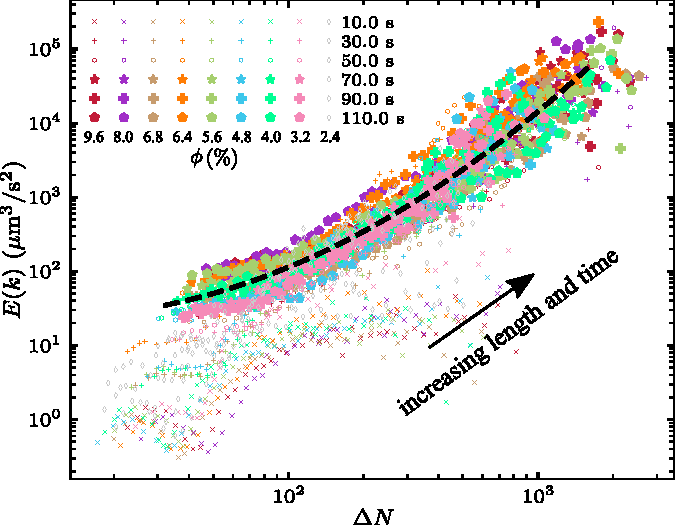
\includegraphics[width=5.5in]{figs/5-GNF/9.pdf}
\caption[Density flow coupling during the transition towards active turbulence]
{
\textbf{Density flow coupling during the transition towards active turbulence.}
Kinetic energy $E$ at various length scales is plotted against number fluctuations $\Delta N/\sqrt N$ at corresponding length scales for bacterial suspensions at volume fractions ranging from 2.4\% to 9.6\% at different times. Different colors indicates samples of different volume fractions. The size and the shape of the markers indicate the time. Small markers stand for early times and large markers stand for late times. In this plot, length scale and time are hidden variables, and their direction of evolving is indicated by a black arrow.
}
\label{fig:GNF-energy-spectra-correlation-transient}
\end{center}
\end{figure}

By comparing the temporal evolution of both GNF and energy spectra during the turbulence transition as shown in Fig.~\ref{fig:GNF-energy-spectra-kinetics}a and b, we find that they are analogous in at least two ways. First, both quantities reach a saturation at $\sim 60$ s. Second, both quantities grow faster at large length scales. Such analogies indicate that GNF and kinetic energy are  closely coupled not only in the steady state of active turbulence, but also during the transient state in the transition to active turbulence.
Motivated by this observation, we plot $\Delta N/\sqrt N$ and $E(k)$ in the same axis for samples of different volume fractions, at different times and length scales in Fig.~\ref{fig:GNF-energy-spectra-correlation-transient}. Indeed, when $\phi>\phi_c$, all the data at different $t$, $\phi$ and length scale $l$ collapse into the same master curve obtained from the steady-state measurements.
This kinetic measurements further suggest that the rise of GNF is governed by the kinetic energy at each corresponding scale.



\section{Conclusion}
In summary, we have measured GNF and energy spectra simultaneously in 3-dimensional bacterial active turbulence. The scaling exponent $\alpha$ we measured is in quantitative agreement with the theoretical prediction of polar-ordered self-propelled particle suspension model.
Our detailed analysis on the turbulent flow fields reveals a strong coupling between flow kinetic energy and GNF, spanning all the length scales down to several swimmer length and up to the vortex size.
Our measurements will contribute to the advancement of quantitative understanding of collective motions and GNF in bacterial active turbulence.
